%================================================================
\chapter{Standard Model of Particles and Multiple Parton Scattering} \label{chap:theo}
%================================================================

This chapter aims to give a theoretical background for this work, an introduction on the Standard Model, which describes the matter building blocks and relevant interactions on the subatomic realm, with exception to the gravity, will be presented. Then the relevant aspects of the QCD (Quantum Chromodynamics) will be discussed, with emphasis to the effective theory NRQCD (Non-Relativistic QCD), which is applied in the context of the quarkonia study. Important concepts on the MPS (Multiple Parton Scattering), which plays an important role on the production of associated production of a quarkonia and a charmed meson will be examined. To finalize, some remarks of the studied channel will be discussed.

\section{Standard Model}

The Standard Model (SM) refers to the set of theories that comprises our current understanding of the particle physics and their interactions \cite{Burgess:2006hbd, perkins_2000}. Even though many phenomena are left without explanation, it passed through many tests from its development on the 70's\footnote{For example, the prediction of particles (e.g. the top quark and the Higgs boson) and their properties with great accuracy.}.

The formulation of the SM is done via the Quantum Field Theory (QFT), in fact, the SM is a QFT of the local gauge group $SU_c(3) \times SU_L(2) \times U_Y(1)$. The SM describes three of the four fundamental interactions, explaining all phenomena in the Universe based on a set of quantum objects with well defined properties often referred to as ``fundamental particles''.

The generators of the symmetry groups form a set of spin-1 bosons that mediates the interactions. The particles associated to the $SU_c(3)$ are called gluons. They carry a charge named color and are massless. The particles that couple with gluons can interact via the strong interaction. The theory that explains the strong interaction is the Quantum Chromodynamics (QCD) and will be further discussed in the Section \ref{sec:QCD}. The group $SU_L(2)$ refers to the weak interaction and the group $U_Y(1)$ the electromagnetic interaction. In the SM, they are unified to give rise to the electroweak interaction which has three massive mediators ($Z, W^+ and W^-$) and one massless (photon). The subscript ``Y'' refers to the electroweak charge from which the electromagnetic charge is defined.

Besides the spin-1 mediators, there are spin-1/2 fundamental particles, which are grouped into doublets, also referred to as generations. These spin-1/2 particles are further divided into quarks, which experience the strong interaction, and leptons, which are not affected by this interaction. 

According to our current knowledge, there are three generations of each, leptons and quarks. 

There are six of leptons: electron ($e$), muon ($\mu$), tau ($\tau$), electron neutrino ($\nu_e$), muon neutrino ($\nu_\mu$) and tau neutrino ($\nu_\tau$)

The hadrons (e.g. the proton, neutron, etc.) are the particles that take side in the strong interactions. They were all found to be bound states of six particles called quarks. Those are: up ($u$), down ($d$), strange ($s$), charm ($c$), bottom ($b$) and top ($t$).

To finalize, there is also a spin-0 field that was introduced in the SM to solve the problem of the particles masses\footnote{The invariance of the theory under $SU_c(3) \times SU_L(2) \times U_Y(1)$ transformations implies that the masses of the particles should be zero.}. This field is responsible to ``give'' mass to the SM particles\footnote{The neutrino mass is still a puzzle. The neutrino oscillation implies that neutrino have mass \cite{Pontecorvo:1957cp, Pontecorvo:1967fh, PhysRevLett.81.1562}. The interaction with Higgs boson requires a right-handed neutrino.}. The masses of the $Z$ and $W^\pm$ bosons are given by the Higgs mechanism, which results in an additional boson with spin 0 called the Higgs boson \cite{PhysRevLett.13.585, PhysRevLett.13.508, PhysRevLett.13.321}. The fermion masses are obtained through a Yukawa interaction between the Higgs and fermion fields.

The Figure \ref{fig:standard_model} summarizes all the fundamental particles of the SM.

\begin{figure}[!htm]{15cm}
\caption{Elementary particles of the Standard Model.}%
\label{fig:standard_model}
\fbox{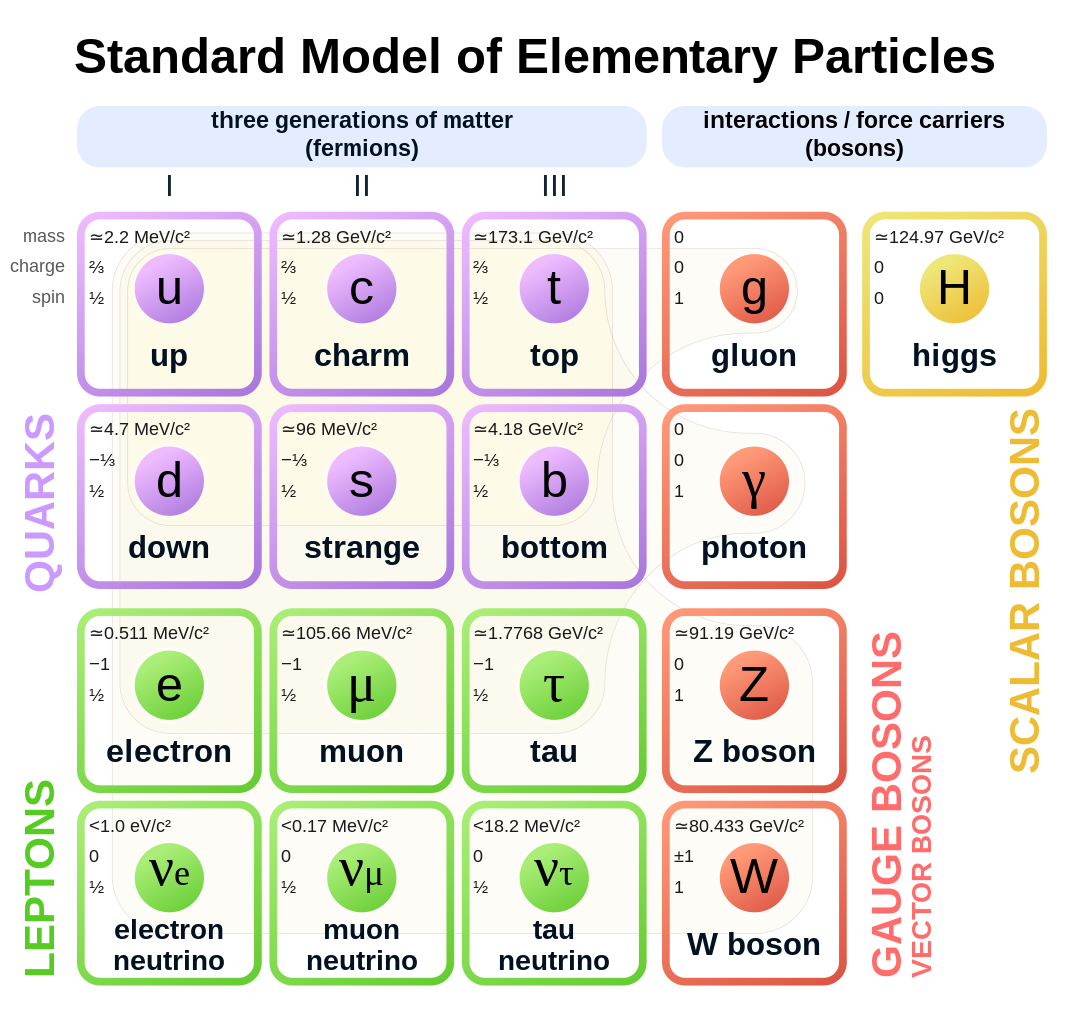
\includegraphics[width=0.98\textwidth]{figures/Standard_Model_of_Elementary_Particles.png}}
\legend{The elementary particles that are part of the Standard Model. Their mass, charge and spin are specified in their box. They are separated in the quarks, leptons, gauge bosons and scalar bosons.}
\source{https://bit.ly/2xk15fQ}
\end{figure}

\section{Quantum Chromodynamics}\label{sec:QCD}

The QCD is the theory of the strong interactions. It is a development from 50 years ago to explain the phenomena of the hadronic matter. The first developments of a theory for the strong interaction began with Murray Gell-Mann and George Zweig to describe the new $\Delta$ particles, the hyperons and the K mesons. Independently, they proposed that the observed hadrons were bound states of particles forming a SU(3) triplet. It was possible to predict new particles as well as explain the difference in the masses of the hadrons, with the quark model called ``eightfold way'' \cite{osti_4008239}.

Later, the color charge was added to the model to explain bound states with three of the same-flavor of quark, which could not exist because the wave function of such state should be anti-symmetric to obey the Pauli principle. The three color charges (red, green and blue) were introduced so that the wave function of the hadrons are anti-symmetric on the color indices.

The number of colors can be confirmed by examination of the cross section of electron-positron annihilation into hadrons, which depends on the square of the charges of the quarks and the number of colors. When comparing to the $e^+e^- \rightarrow \mu^+\mu^-$ annihilation\footnote{This is a naive approximation, and can be corrected by higher order perturbative QCD calculations.}
\begin{equation}
    R = \frac{\sigma(e^+e^- \rightarrow \text{hadrons})}{\sigma(e^+e^- \rightarrow \mu^+\mu^-)} = n_c \times \sum_q Q_q^2\,
\end{equation}
where $n_c$ is the number of colors, $Q$ is the electric charge and the subscript $q$ is the quark flavour. Figure \ref{fig:Rsigma} shows the measurement of R in electron-positron collisions.

\begin{figure}[!htm]{15cm}
\caption{Cross section and R in electron-positron collisions.}%
\label{fig:Rsigma}
\fbox{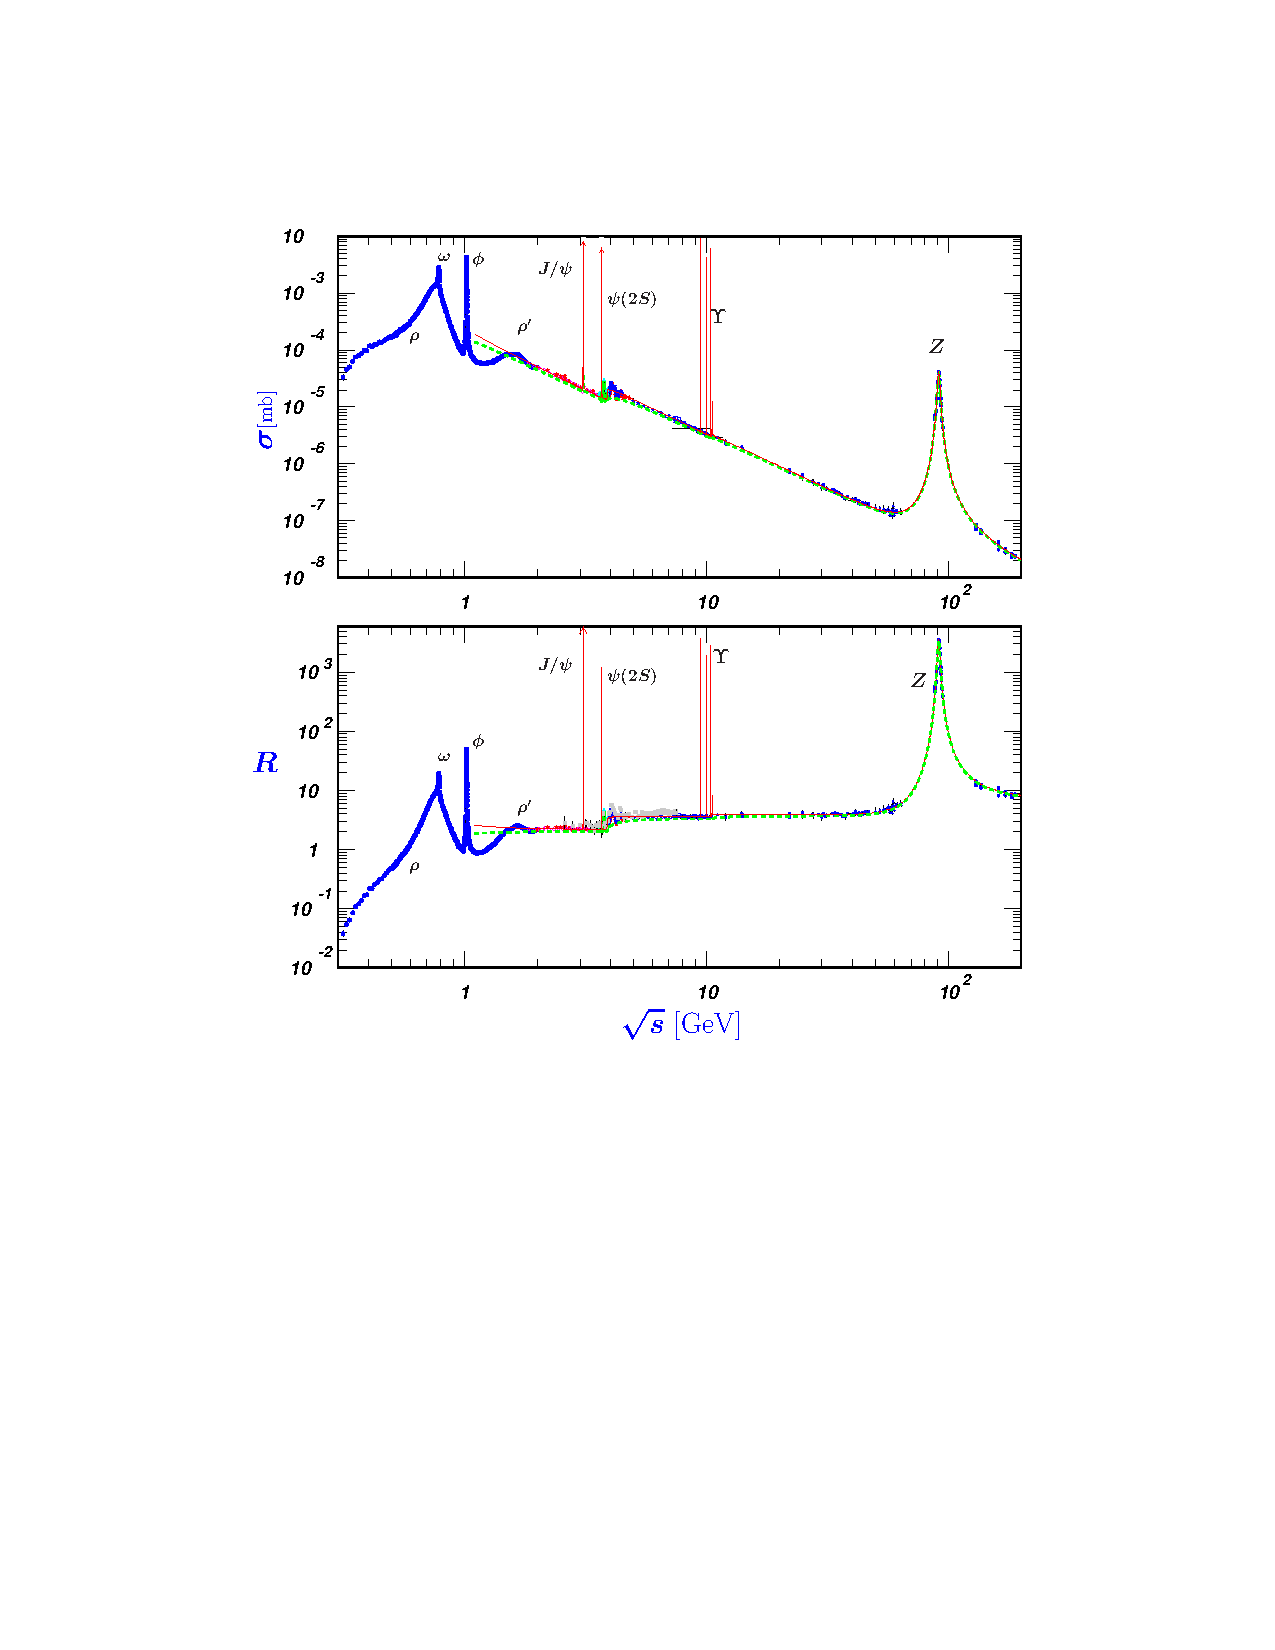
\includegraphics[width=0.8\textwidth]{figures/rpp2022-sigma_R_ee.pdf}}
\legend{Data (blue) on the total cross section of $\sigma(e^+e^- \rightarrow \text{hadrons})$ and the ratio $R = \sigma(e^+e^- \rightarrow \text{hadrons})/\sigma(e^+e^- \rightarrow \mu^+\mu^-)$. The broken curve (green) is a naive quark-parton model prediction, and the solid one (red) is 3-loop perturbative QCD prediction.}
\source{\cite{Workman:2022ynf}}
\end{figure}

The QCD was introduced to explain the quark model and its properties as a non-abelian SU(3) gauge theory \cite{Fritzsch:1973pi}. The Lagrangian of QCD is
\begin{equation}
    \mathcal{L}_{QCD} = \sum_f \overline{\psi}_{f,a}(i\delta_{ab}\slashed{D} - m_f\delta_{ab})\psi_{f,b} - \frac{1}{4}G^a_{\mu\nu}G^{a\mu\nu},
\end{equation}
where $\psi_{f, a}$ are quark field spinors for a quark of flavor q, mass $m_f$ and a color-index $a$ that runs from a = 1 to 3 (for red, green and blue). The $\slashed{D}$ is the covariant derivative, it contains the coupling between the quark and gluons fields 
\begin{equation}
    \slashed{D} = \gamma^\mu(\partial_\mu - i g_s A^a_\mu),
\end{equation}
where $A_\mu$ represents the gluon fields, which are generators of the SU(3) gauge group. The $g_s$ is the gauge coupling constant. The second term of the Lagrangian represents the kinetic term of the gluonic fields. They are expressed in terms of the field strength tensor $G^a_{\mu\nu}$ which is written in terms of the gluon fields as
\begin{equation}
    G^a_{\mu\nu} = \partial_\mu A^a_\nu - \partial_\nu A^a_\mu + g_sf^{abc}A^b_\mu A^c_\nu,
\end{equation}
where $f^{abc}$ are the structure constants of the SU(3) group. 

The coupling of the gluon fields with themselves occurs because the gluons carry color. Therefore, the QCD Feynman rules admit vertexes with three and four gluons as shown in Fig. \ref{fig:QCDvertex}. In comparison, there is only one vertex in the QED Feynman rules, with two fermions and one photon, since the photon caries no electric charge.

\begin{figure}[!htm]{15cm} 
\caption{QCD Feynman diagram vertex.}%
\label{fig:QCDvertex}
\fbox{
\begin{tabular}{ccc}
\begin{tabular}{c}
    \feynmandiagram [horizontal=a to b] { i1[particle=\(q\)] -- [fermion] a -- [fermion] i2[particle=\(q\)], a -- [gluon] b[particle=\(g\)],
    };
\end{tabular} & 
\begin{tabular}{c}
    \feynmandiagram [horizontal=a to b] { i1[particle=\(g\)] -- [gluon] a -- [gluon] i2[particle=\(g\)], a -- [gluon] b[particle=\(g\)],
    };
\end{tabular} & 
\begin{tabular}{c}
    \begin{tikzpicture}
        \begin{feynman}
            \vertex(a) ;
            \vertex[above left=of a](i1) {\(g\)};
            \vertex[below left=of a](i2) {\(g\)};
            \vertex[above right=of a](i3) {\(g\)};
            \vertex[below right=of a](i4) {\(g\)};
            \diagram*{
                (i1) -- [gluon] (a) -- [gluon] (i2),
                (i3) -- [gluon] (a) -- [gluon] (i4),
            };
        \end{feynman}
    \end{tikzpicture}
\end{tabular}
\end{tabular}
}
\legend{The allowed vertex in QCD. Besides the quark-gluon coupling represented by the first diagram from left to right, resembling the QED vertex, there are two more diagrams representing gluon-gluon interaction.}
\end{figure}

Only color-singlet (i.e. color neutral) particles are observed, therefore quarks and gluons are not directly detected free in the Nature. There are two types of hadrons which are commonly probed in experiments - the mesons, formed by the combination of a quark and a antiquark
\begin{equation}
    (q\overline q) \rightarrow (q_r \overline q_r + q_g \overline q_g + q_b \overline q_b)
\end{equation}
and the baryons formed by a combination of three quarks or three antiquarks
\begin{equation}
    (qqq) \rightarrow (q_r q_g q_b - q_g q_r q_b + q_b q_r q_g - q_r q_b q_g + q_g q_b q_r - q_b q_g q_r).
\end{equation}
Other kinds of states, such as tetraquarks or pentaquarks (4 and 5 quark and antiquark bound states, respectively, commonly called exotic) are possible \cite{Gell-Mann:1964ewy, Zweig:1964jf}, a list of such states observed in LHC can be found in \cite{LHCb-FIGURE-2021-001-report}. Also, gluon-gluon bound states are possible, known as glueball or gluonium, but were never observed \cite{Mathieu:2008me}. 

QCD has two very unique properties, asymptotic freedom and color confinement. Asymptotic freedom states that in the limit of high energies, the coupling constant of the QCD ($\alpha_s = \frac{g_s}{4\pi}$) becomes small \cite{PhysRevLett.30.1343, PhysRevLett.30.1346} and it can be treated perturbatively. Measurements of $\alpha_s$ are shown in Figure \ref{fig:couplingQCD}, which illustrates this behavior. Color confinement express the fact that free quarks are not observed. It is understood as a consequence of gluon self-interaction and the consequent increase of potential energy due to the color field as two quarks in a hadron are separated.

\begin{figure}[!htm]{15cm}
\caption{QCD coupling constant.}%
\label{fig:couplingQCD}
\fbox{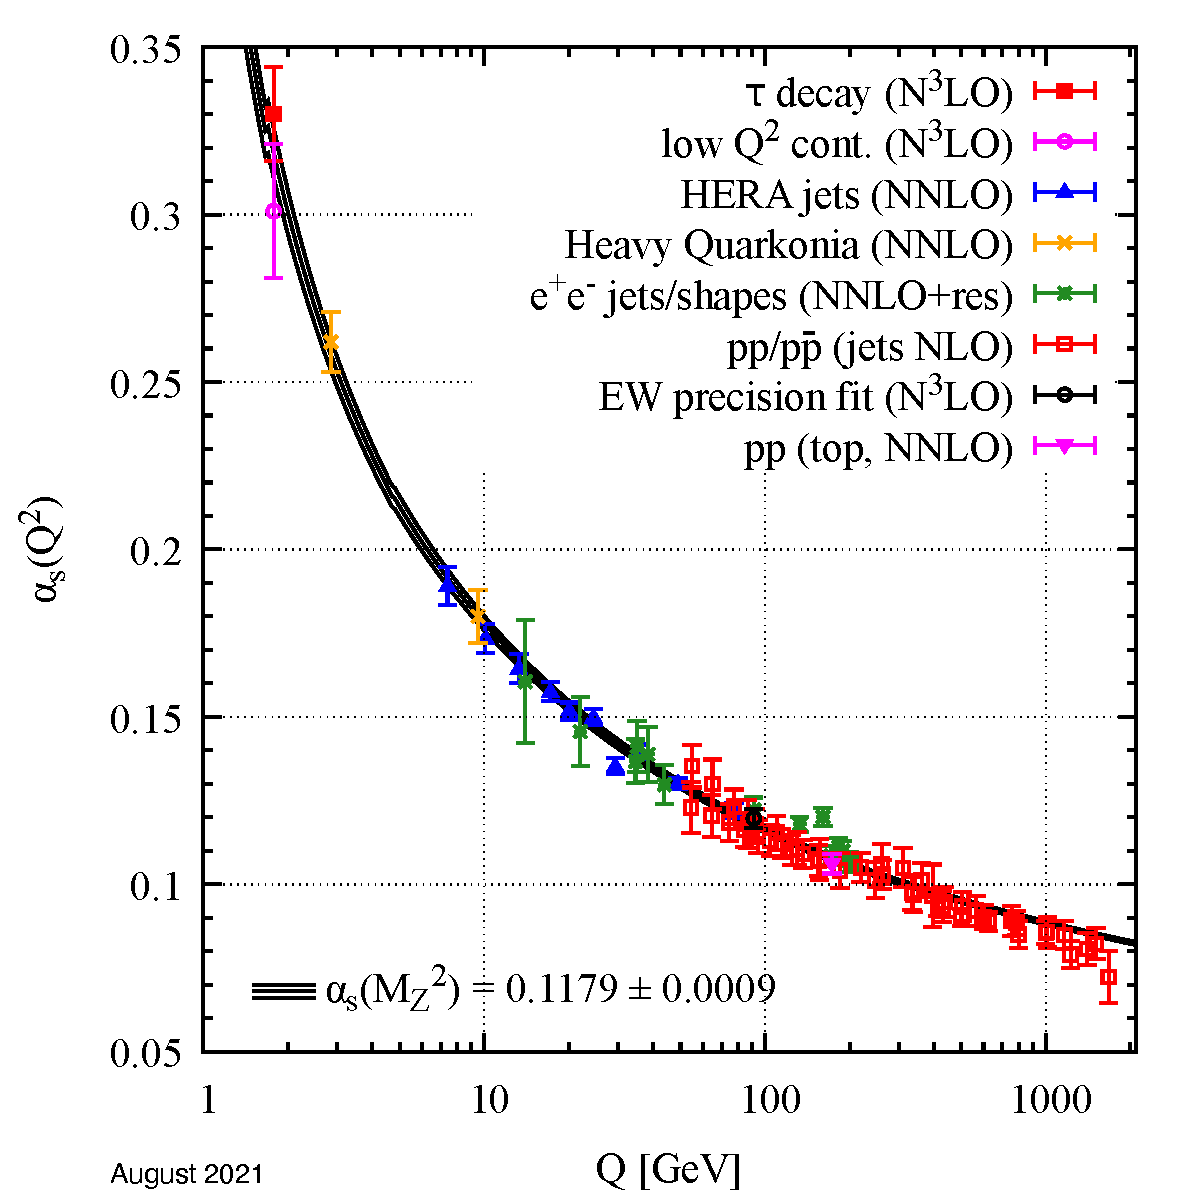
\includegraphics[width=0.8\textwidth]{figures/alphas-v-Q-2021.pdf}}
\legend{Summary of measurements of $\alpha_s$ as a function of the energy scale Q. The respective degree of QCD perturbation theory used in the extraction of $\alpha_s$ is indicated in brackets (NLO: next-to-leading order; NNLO: next-to-next-to-leading order; NNLO+res.: NNLO matched to a resummed calculation; N$^3$LO: next-to-NNLO)}
\source{\cite{Workman:2022ynf}}
\end{figure}

\section{Quarkonia}

The quarkonia are mesons made of a heavy quark and antiquark of the same flavour. The possible quarkonium states are the $c\overline{c}$, the charmonium, and $b\overline{b}$, the bottomonium. Light mesons (u, d and s) form physical quark-antiquark states\footnote{The $\eta$, $\eta^\prime$, and $\pi^0$ mesons.} but, because of their small mass, they are actually quantum mechanical mixtures of such states. Finally, the top quark quarkonium is not expected to be found, because, due to its very high mass, the top quark decays through electroweak interaction before a bound state can be formed, but there are some signatures that could be explored in the search for the toponium \cite{Fuks:2021xje}.

The special property of the quarkonia is that they form a bound-state with radius much lower than confinement scale, thus the QCD coupling constant has lower values, so that these particles can be treated perturbatively, which leads to states that are very similar to the electromagnetic particle-antiparticle systems \cite{Burgess:2006hbd}, the positronium and the muonium, from which the quarkonium name derives. Furthermore, because they are made of heavy quarks they form non-relativistic states, which are very well treated by a effective theory called NRQCD.

The $c\overline{c}$ and $b\overline{b}$ bound states may be classified with respect to their principal quantum number, $n$, angular momentum quantum numbers, $l$ and $m$, and spin quantum numbers, $s$ and $s_z$, using the same spectroscopic notation used in atoms. Figure \ref{fig:qq_spectrum} shows the quarkonium spectrum.

\begin{figure}[!htm]{15cm}
  \caption{Quarkonium spectrum.} 
  \label{fig:qq_spectrum}
  \subfloat[][]{\label{subfig:cc_spectrum}%
    \fbox{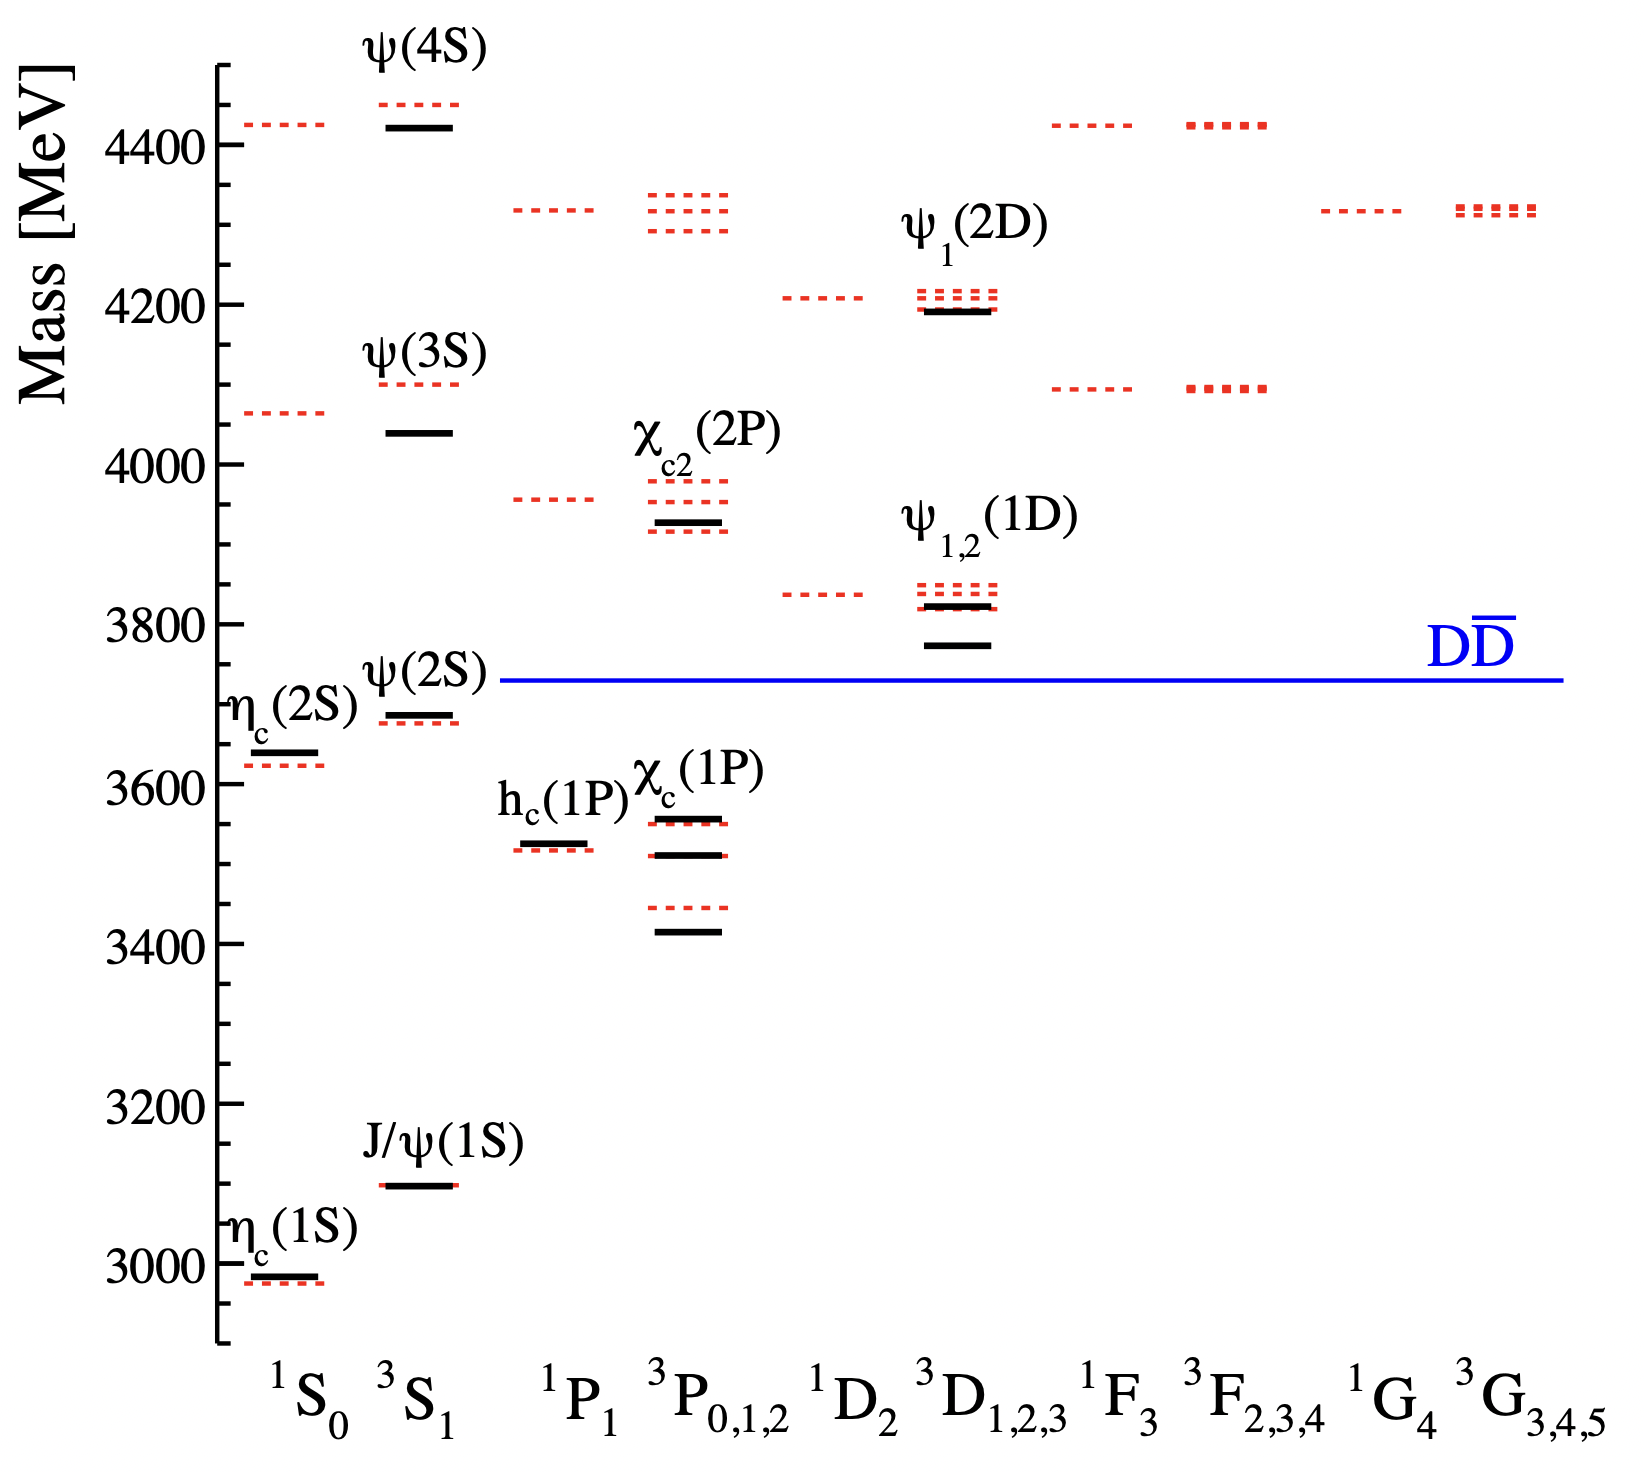
\includegraphics[width=0.45\textwidth]{figures/cc_spectrum.png}}}\hfill
  \subfloat[][]{\label{subfig:bb_spectrum}%
    \fbox{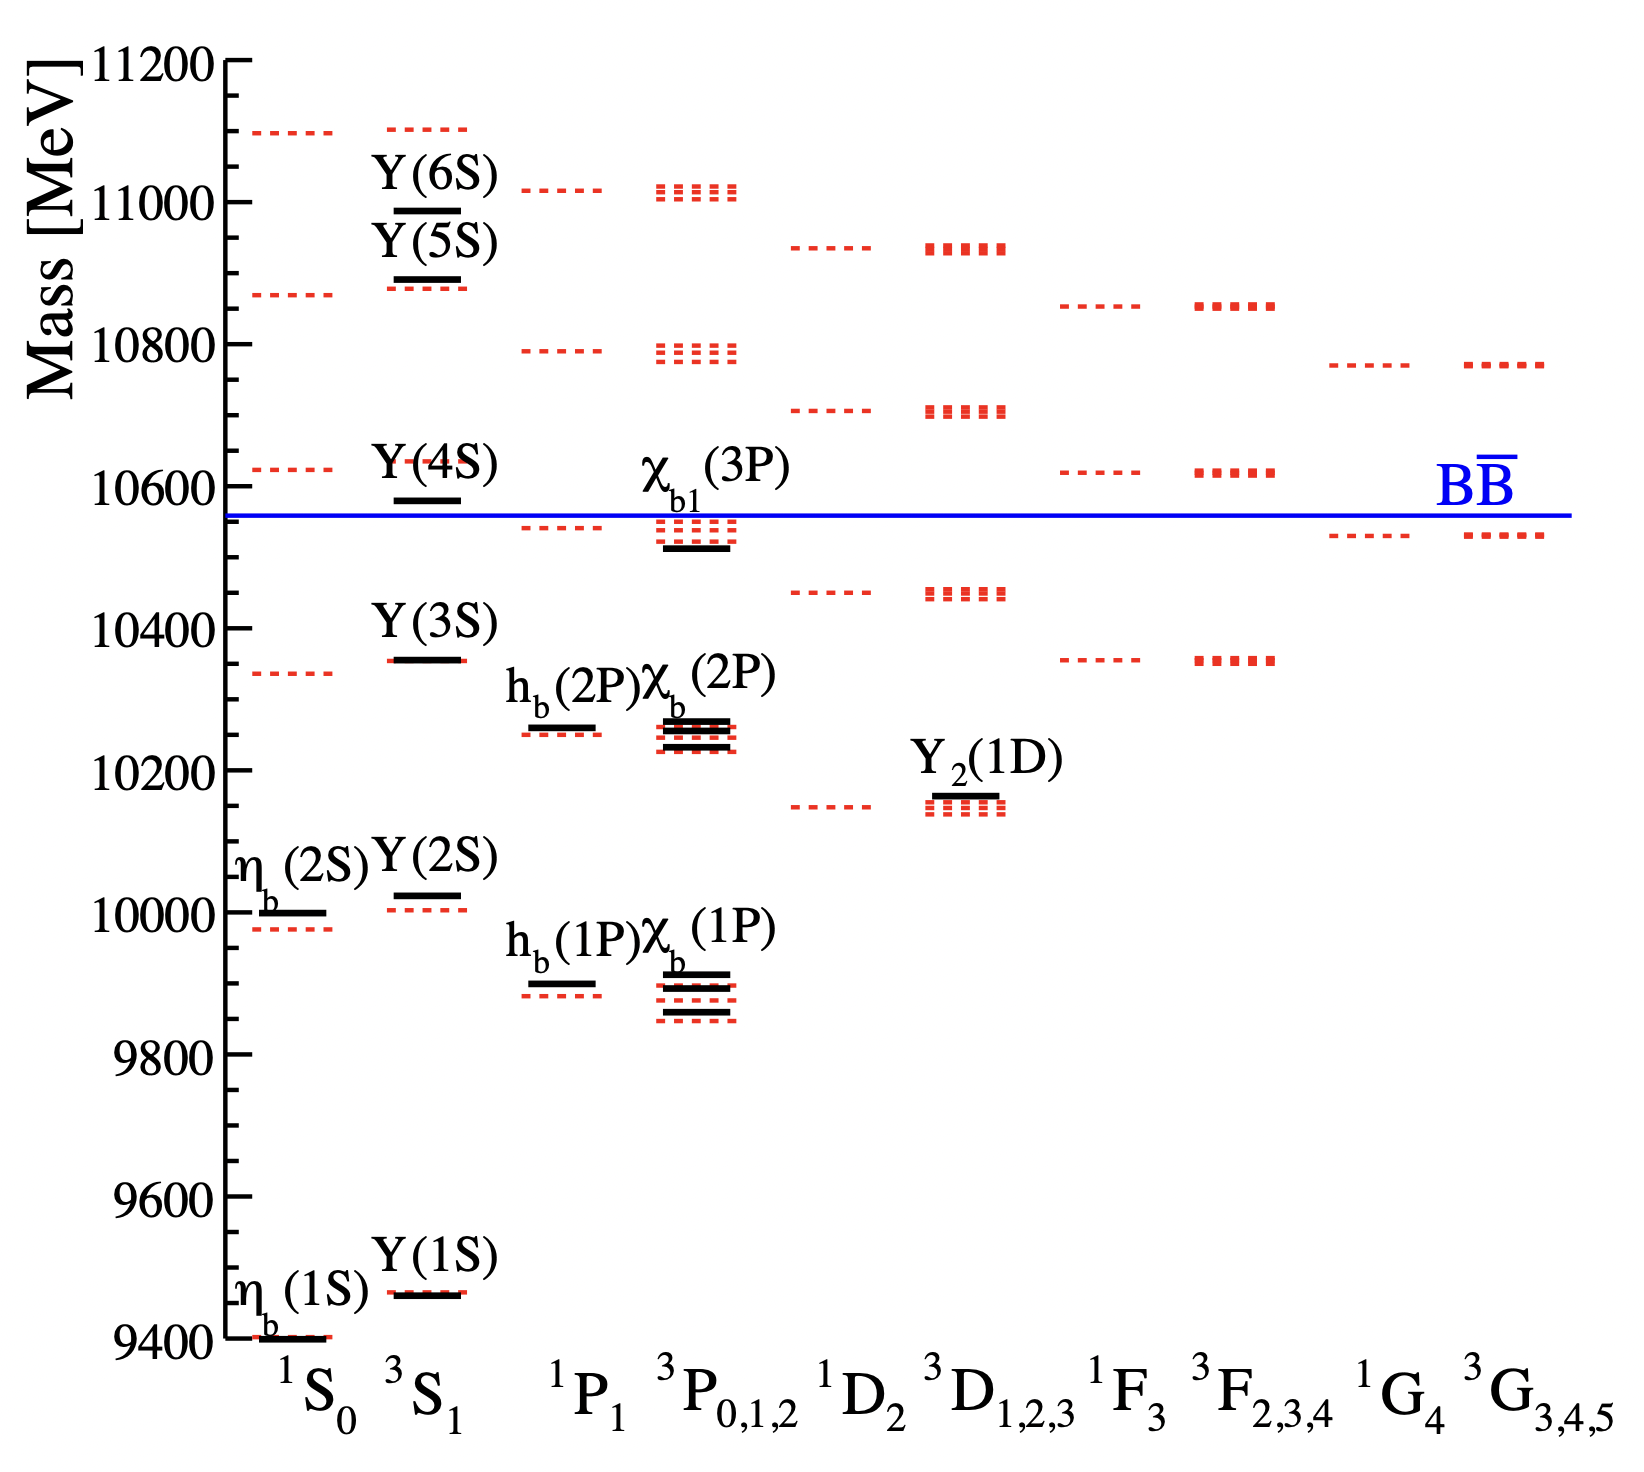
\includegraphics[width=0.45\textwidth]{figures/bb_spectrum.png}}}\\
  \legend{Current status of the charmonium (a) and bottomonium (b) spectra. The dashed lines indicate the expected states and their masses. The solid lines indicates the experimentally established quarkonia states. The open-flavor threshold is indicated in the blue line.}
  \source{\cite{RevModPhys.90.015003}}
\end{figure}

The discovery of the J/$\psi$, in 1974 \cite{E598:1974sol, SLAC-SP-017:1974ind}, allowed to identify the charm quark, confirming the quarks as real particles and not mathematical entities to explain the hadrons. This triggered many changes in the understanding of particle physics which is today known as November Revolution. Later, the $\Upsilon$ meson was discovered in 1977 \cite{E288:1977xhf}, the first particle containing b quarks.

Still today, the quarkonia are of very interest in particle physics, because they are easy to be treated experimentally and have high yields in the LHC energy scale. They appear as products of decays of exotic states \cite{CMS:2013jru, LHCb:2021uow, LHCb:2021vvq}, B mesons and Higgs boson \cite{ATLAS:2015vss} and can hint properties of the Quark-Gluon Plasma \cite{Matsui:1986dk, Wolschin:2016oua}.

\section{Multiple Parton Scattering}

Protons are not elementary particles, they are formed by a bound state of uud quarks, called valence quarks, the gluons that bind the valence quarks together and the sea quarks and antiquarks, which are formed by the interaction of the gluons in the protons. All of them are collectively referred to as partons.

Therefore, as opposed to the electron-positron collision, one cannot determine the initial states of a proton-proton (pp) collision and the calculation of the perturbative cross sections are determined be the factorization theorem \cite{Collins:1989gx}. If one parton from each proton interact, cross section can be determined as
\begin{equation}\label{eq:SPSxsec}
    \sigma_{A} = \sum_{i,j}\int dx_i \; dx_j \; f_i(x_i, \mu_F) \; f_j(x_j, \mu_F) \cdot \Hat{\sigma}_{i,j}^X(x_i, x_j, \mu_F)  
\end{equation}
where, $i$ and $j$ are the interacting partons, $x_i$ ($x_j$) is the momentum fraction carried by the parton $i$ ($j$), $f(x, \mu_F)$ is the parton distribution function (PDF), which is defined as the probability density for finding a parton with a certain longitudinal momentum fraction $x$ at factorization scale $\mu_F$ and $\Hat{\sigma}$ is the partonic cross section that can be calculated by the perturbative QCD (pQCD). The PDFs are the non-perturbative part of the Eq. \ref{eq:SPSxsec} and are determined experimentally \cite{NNPDF:2017mvq} and are shown in Fig. \ref{fig:NNLOPDFs}.

\begin{figure}[!htm]{15cm} 
\caption{NNLO Parton Distribution Functions.}%
\label{fig:NNLOPDFs}
\fbox{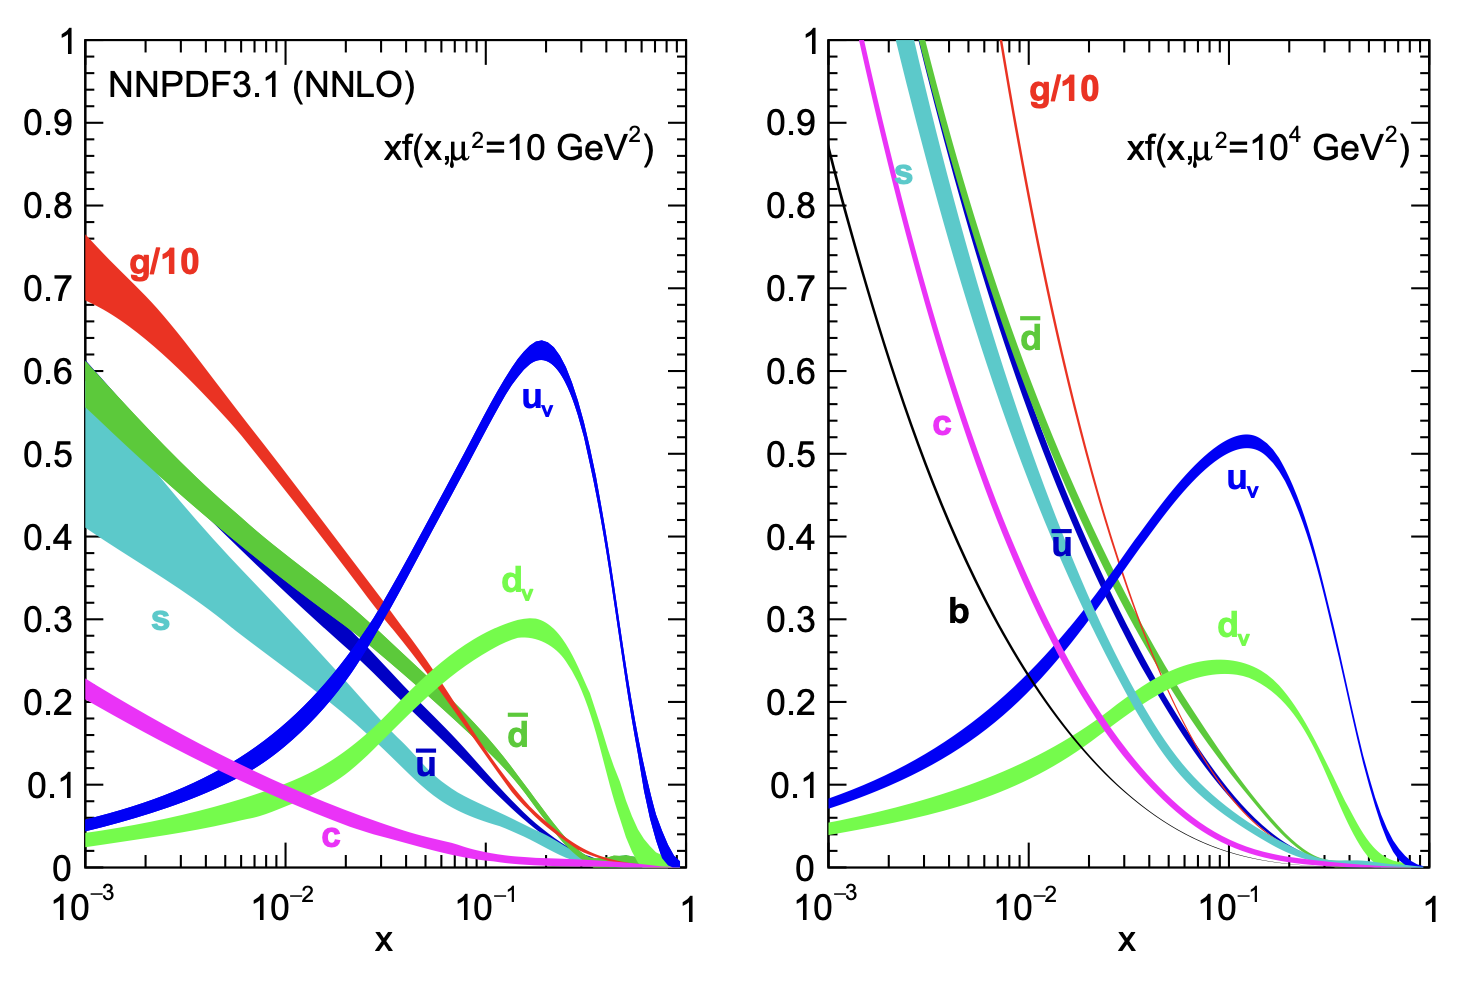
\includegraphics[width=0.9\textwidth]{figures/NNLO_PDFs.png}}
\legend{NNLO Parton distribution functions determined for $\mu_F^2 =$ 10 GeV$^2$ (left) and 10$^4$ GeV$^2$ (right)}
\source{\cite{NNPDF:2017mvq}}
\end{figure}

It is also possible that more than one parton from each proton take part in the process, giving rise to more than one hard interaction, a process known as Multiple Parton Scattering (MPS). In the MPS context, the pp interaction with one hard interaction is called Single Parton Scattering (SPS) and first extension is the Double Parton Scattering (DPS), where two hard interactions happen. Figure \ref{fig:SPSxDPS} shows the SPS and DPS examples.

\begin{figure}[!htm]{15cm}
  \caption{Single Parton Scattering and Double Parton Scattering sketches.} 
  \label{fig:SPSxDPS}
  \subfloat[][]{\label{subfig:SPS}%
    \fbox{
\begin{tikzpicture}
\begin{feynman}
\vertex(i1) {\(p\)};
\vertex[below=3cm of i1](i2) {\(p\)};
\vertex[blob, right=2cm of i1](h1) {};
\vertex[above=.15 of h1](h12) {};
\vertex[below=.15 of h1](h13) {};
\vertex[blob, right=2cm of i2](h2) {};
\vertex[above=.15 of h2](h22) {};
\vertex[below=.15 of h2](h23) {};
\vertex[blob, below right=2.12cm of h1](a) {};
\path (a) ++ (00:2) node[vertex] (o2);
\path (a.+30-|o2.center) node[vertex] (o1);
\path (a.-30-|o2.center) node[vertex] (o3);
\path (h1) ++ (00:2) node[vertex] (hf2);
\path (h1.+30-|hf2.center) node[vertex] (hf3);
\path (h1.+60-|hf2.center) node[vertex] (hf4);
\path (h2) ++ (00:2) node[vertex] (hf5);
\path (h2.-30-|hf4.center) node[vertex] (hf6);
\path (h2.-60-|hf4.center) node[vertex] (hf7);
\path (i1.+30-|h12.center) node[vertex] (i12);
\path (i1.-30-|h13.center) node[vertex] (i13);
\path (i2.+30-|h22.center) node[vertex] (i22);
\path (i2.-30-|h23.center) node[vertex] (i23);

\diagram* {
    (i1) -- [fermion] (h1) -- (a),
    (i1.+30) -- [fermion] (h12),
    (i1.-30) -- [fermion] (h13),
    (i2.+30) -- [fermion] (h22),
    (i2.-30) -- [fermion] (h23),
    (i2) -- [fermion] (h2) -- (a) -- (o2),
    (a.-30) -- (o3),
    (a.+30) -- (o1),
    (h1) -- [fermion] (hf2),
    (h1.+30) -- [fermion] (hf3),
    (h1.+60) -- [fermion] (hf4),
    (h2) -- [fermion] (hf5),
    (h2.-30) -- [fermion] (hf6),
    (h2.-60) -- [fermion] (hf7),
};
\end{feynman}
\end{tikzpicture}
    }}\hfill
  \subfloat[][]{\label{subfig:DPS}%
    \fbox{
\begin{tikzpicture}
\begin{feynman}
\vertex(i1) {\(p\)};
\vertex[below=3cm of i1](i2) {\(p\)};
\vertex[blob, right=2cm of i1](h1) {};
\vertex[above=.15 of h1](h12) {};
\vertex[below=.15 of h1](h13) {};
\vertex[blob, right=2cm of i2](h2) {};
\vertex[above=.15 of h2](h22) {};
\vertex[below=.15 of h2](h23) {};
\vertex[blob, below right=of h1](a) {};
\vertex[blob, above right=of h2](b) {};
\path (a) ++ (00:2) node[vertex] (o2);
\path (a.+30-|o2.center) node[vertex] (o1);
\path (a.-30-|o2.center) node[vertex] (o3);
\path (b) ++ (00:2) node[vertex] (o5);
\path (b.+30-|o5.center) node[vertex] (o4);
\path (b.-30-|o5.center) node[vertex] (o6);
\path (h1) ++ (00:2) node[vertex] (hf2);
\path (h1.+30-|hf2.center) node[vertex] (hf3);
\path (h1.+60-|hf2.center) node[vertex] (hf4);
\path (h2) ++ (00:2) node[vertex] (hf5);
\path (h2.-30-|hf4.center) node[vertex] (hf6);
\path (h2.-60-|hf4.center) node[vertex] (hf7);
\path (i1.+30-|h12.center) node[vertex] (i12);
\path (i1.-30-|h13.center) node[vertex] (i13);
\path (i2.+30-|h22.center) node[vertex] (i22);
\path (i2.-30-|h23.center) node[vertex] (i23);

\diagram* {
    (i1) -- [fermion] (h1) -- (a),
    (i1.+30) -- [fermion] (h12),
    (i1.-30) -- [fermion] (h13),
    (i2.+30) -- [fermion] (h22),
    (i2.-30) -- [fermion] (h23),
    (i2) -- [fermion] (h2) -- (a) -- (o2),
    (h1) -- (b),
    (h2) -- (b),
    (a.-30) -- (o3),
    (a.+30) -- (o1),
    (b.-30) -- (o6),
    (b.+30) -- (o4),
    (b) -- (o5),
    (h1) -- [fermion] (hf2),
    (h1.+30) -- [fermion] (hf3),
    (h1.+60) -- [fermion] (hf4),
    (h2) -- [fermion] (hf5),
    (h2.-30) -- [fermion] (hf6),
    (h2.-60) -- [fermion] (hf7),
};
\end{feynman}
\end{tikzpicture}
    }}\\
  \legend{A comparison of the Single Parton Scattering (a) and Double Parton Scattering (b). The difference between the two are the number of partons coming from each proton. The hadrons formed in (b) are uncorrelated, and have different kinematic distributions than (a)}
\end{figure}

The factorization can also be used in the MPS. For the DPS, the cross section is calculated by the formula \cite{gaunt2010double}
\begin{equation}\label{eq:DPSxsecfull}
\begin{split}
    \sigma_{AB}^{DPS} = \frac{m}{2} \sum_{i,j,k,l}\int & \Gamma_{ij}(x_1, x_2, b, \mu_1, \mu_2) \; \Hat{\sigma}^A_{ik}(x_1, x_1^\prime, \mu_1) \; \Hat{\sigma}_{jl}^B(x_2, x_2^\prime, \mu_2) \\ & \times \Gamma_{kl}(x_1^\prime, x_2^\prime, b, \mu_1, \mu_2) \; dx_1\; dx_2\; dx_1^\prime\; dx_2^\prime\; d^2b,
\end{split}
\end{equation}
where the $m$ is a double count factor, m equals 1 if process A = process B and 2 otherwise. The $\Gamma_{ij}(x_1, x_1, b, \mu_1, \mu_2)$ are the generalized double parton distributions. They may be interpreted as the inclusive probability distributions to find a parton i with longitudinal momentum fraction $x_1$ at scale $\mu_1$ in the proton, in addition to a parton j with longitudinal momentum fraction $x_2$ at scale $\mu_2$, with the two partons separated by a transverse distance b. And finally the $\Hat{\sigma}$ is the parton-level cross section.

The multi-parton PDFs should depend on all the possible correlations between partons, such as color and flavour interactions as well as spatial and kinematics correlations. Currently there is no theoretical model capable to describe its phenomenology. So, as a simplification to the model, it is assumed that the $\Gamma_{ij}$ can be separated in two components, representing the longitudinal and transverse components
\begin{equation}
    \Gamma_{ij}(x_1, x_2, b, \mu_1, \mu_2) = D_{ij}(x_1, x_2, \mu_1, \mu_2)\cdot F(b).
\end{equation}

The correlations in the transverse plane are very significant - as they must bind the two partons together within the same hadron. On the other hand, the correlations in the longitudinal plane are typically ignored with the assumption that, at least for small $x_i$ values the longitudinal momenta correlations are small\footnote{At LHC energy scale, the fraction of partons with small $x$ is large.} \cite{gaunt2010double}. Therefore, $\Gamma_{ij}$ is taken as the product of the single parton distribution functions $f_i$ and $f_j$
\begin{equation}\label{eq:simpdPDF}
    \Gamma_{ij}(x_1, x_2, b, \mu_1, \mu_2) = f_j(x_1, \mu_1) \cdot f_i(x_2, \mu_2) \cdot F(b).
\end{equation}

Under those simplifications, the DPS cross section can be expressed in terms of the SPS cross sections by plugging Eq. \ref{eq:simpdPDF} in \ref{eq:DPSxsecfull}
\begin{equation} \label{eq:xsecDPS}
    \sigma_{AB}^{DPS} = \frac{m}{2} \frac{\sigma_A^{SPS} \cdot \sigma_B^{SPS}}{\sigma_{eff}},
\end{equation}
where $m$ is one if $A = B$ and two if $A \neq  B$, $\sigma^{SPS}_A$ is the inclusive cross section of the process A and has the same formula from Eq. \ref{eq:SPSxsec}. The $\sigma_{eff}$ is written as
\begin{equation}\label{eq:sigmaeff}
    \sigma_{eff} = \left[ \int d^2b (F(b))^2 \right]^{-1}
\end{equation}
and it is a parameter characterizes the effective spatial area of the parton-parton interactions. Figure \ref{fig:sigmaeff_measurements} shows a summary of measurements of $\sigma_{eff}$ done by many experiments \cite{afs1987double,alitti1991study,abe1993study,cdf1997double,abazov2010double,aaij2012observation,aad2013measurement,chatrchyan2014study,abazov2014double,abazov2014observation,alconada2015observation,aaboud2016study,aaij2016production,abazov2016study,abazov2016evidence,aaij2017measurement,atlas2017measurement,khachatryan2017observation,sirunyan2018constraints}. The results shows some deviations on the measured effective cross section, which should be independent of final state.

\begin{figure}[!htm]{15cm} 
\caption{Measurements and limits on the $\sigma_{eff}$.}%
\label{fig:sigmaeff_measurements}
\fbox{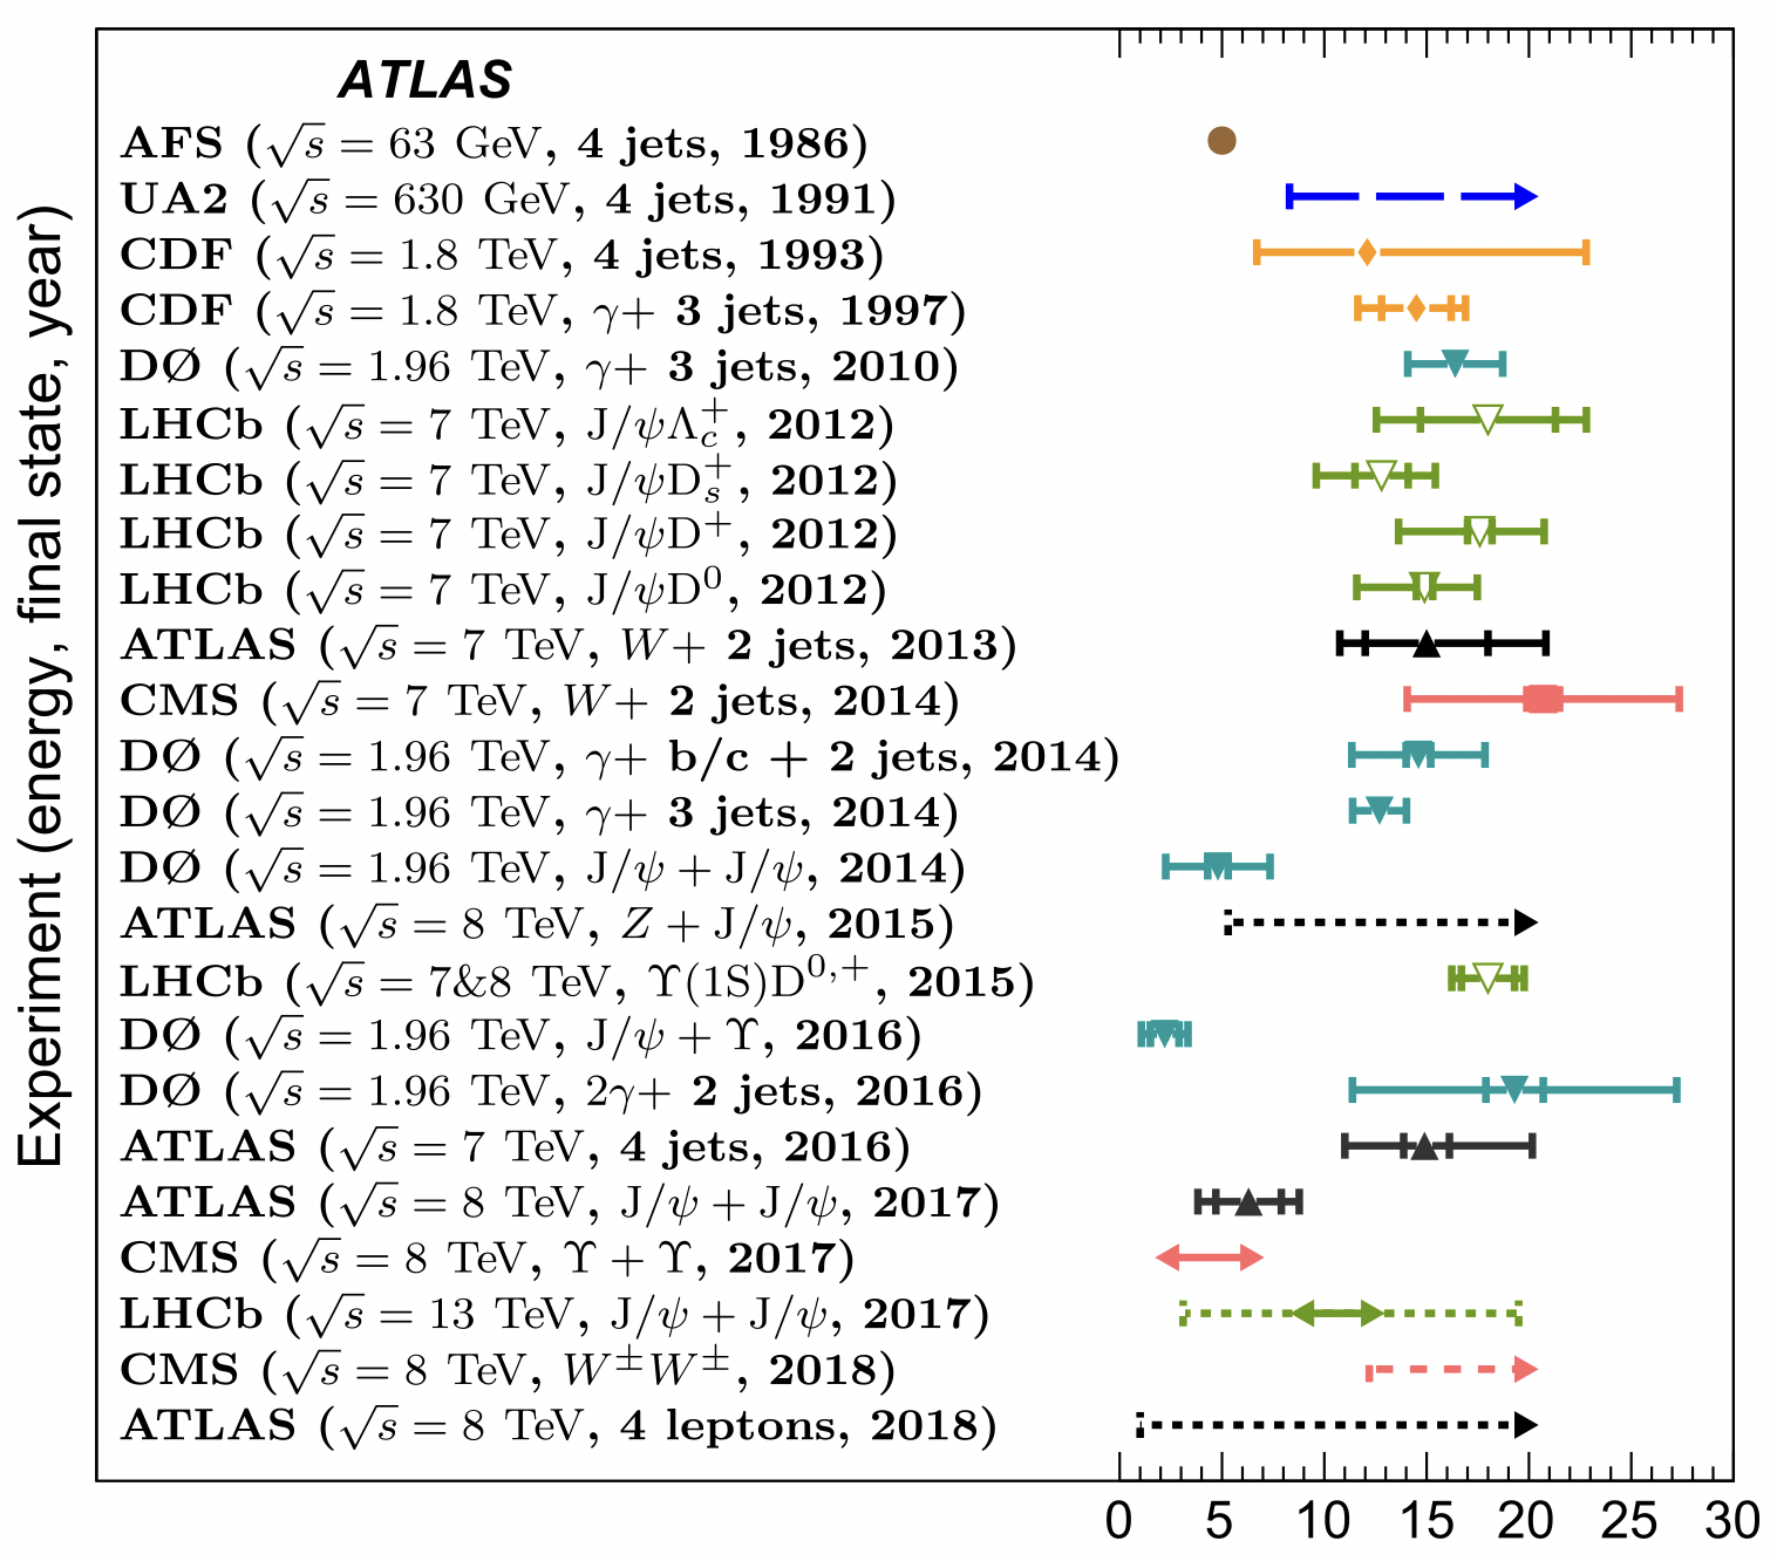
\includegraphics[width=0.68\textwidth]{figures/sigma_eff_measurements.png}}
\legend{Summary of measurements and limits on the $\sigma_{eff}$ determined by many experiments \cite{afs1987double,alitti1991study,abe1993study,cdf1997double,abazov2010double,aaij2012observation,aad2013measurement,chatrchyan2014study,abazov2014double,abazov2014observation,alconada2015observation,aaboud2016study,aaij2016production,abazov2016study,abazov2016evidence,aaij2017measurement,atlas2017measurement,khachatryan2017observation,sirunyan2018constraints}.}
\source{\cite{ATLAS:2018zbr}}
\end{figure}

The MPS is of great interest in the experiments as it can be a important contribution to background in multiparticle final-state processes. In high energy experiments, the MPS contribution is large, and can even overtake the SPS one \cite{Luszczak:2011zp}. Figure \ref{fig:SPSvsDPS} show the contribution of SPS and DPS to $c \bar c$ production, it is possible to see that at high enough center-of-mass energy, the DPS contribution is larger than SPS.

\begin{figure}[!htm]{15cm} 
\caption{Total LO $c \bar{c}$ cross section for SPS and DPS as a function of $\sqrt{s}$.}%
\label{fig:SPSvsDPS}
\fbox{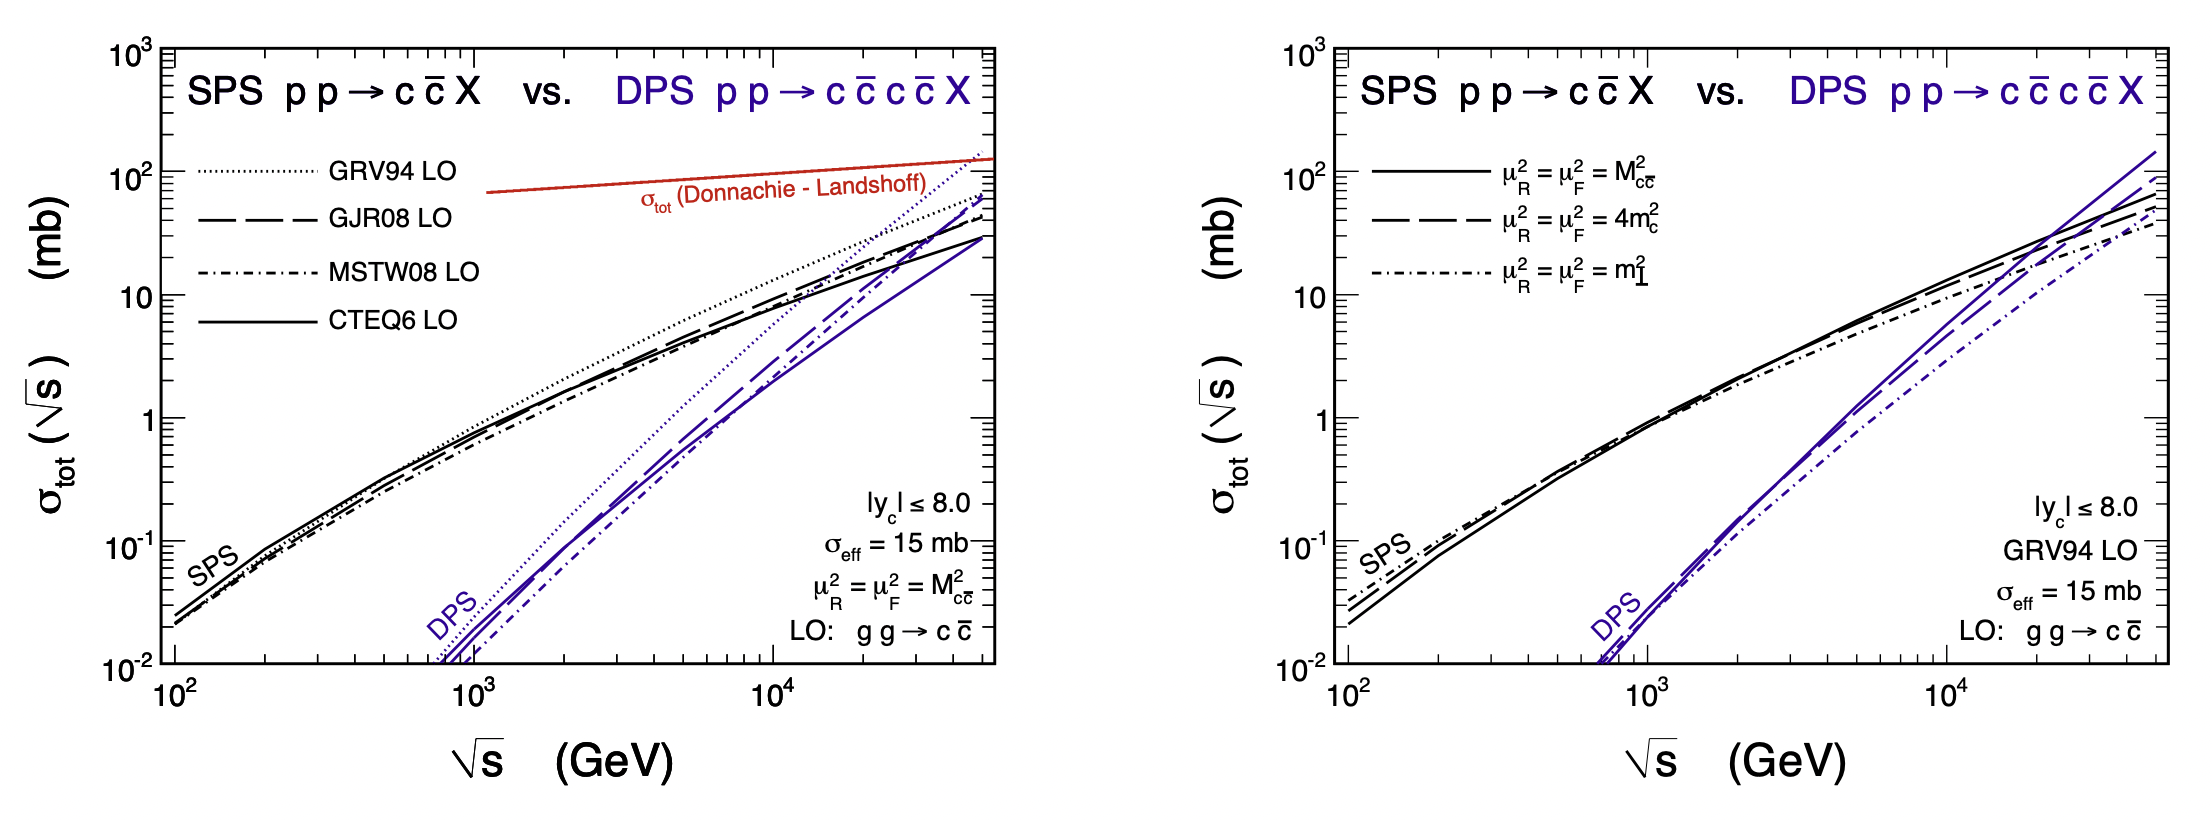
\includegraphics[width=0.98\textwidth]{figures/DPSvsSPS.png}}
\legend{Total LO cross section for SPS and DPS as a function of center-of-mass energy (left) and uncertainties due to the choice of (factorization, renormalisation) scales (right).}
\source{\cite{Luszczak:2011zp}}
\end{figure}

\section{Associated production of \texorpdfstring{$\Upsilon$}{Y } and Open Charm} \label{sec:theoryY+D}

The associated production of $\Upsilon$ and open charm is an interesting channel to investigate DPS \cite{Lansberg:2019adr} as it is expected that the SPS contribution is small. There is an experimental measurement from LHCb collaboration in 2015 \cite{aaij2016production} in which they concluded that the DPS cross section is at least 10 times higher than the SPS one, as expected from the theoretical study \cite{Berezhnoy:2015jga}. 

Under the hypothesis of the dominance of the DPS, LHCb extracted the values for the fiducial and effective cross section
\begin{equation}
\begin{split}
    BR_{Y \rightarrow \mu^+\mu^-} \times \sigma^{Y(1S)D^0}_{\sqrt{s}=7\, \text{TeV}} &= 155 \pm 21 (\text{stat}) \pm 7(\text{syst}) \, \text{pb}, \\
    BR_{Y \rightarrow \mu^+\mu^-} \times \sigma^{Y(1S)D^+}_{\sqrt{s}=7\, \text{TeV}} &= 82 \pm 19 (\text{stat}) \pm 5(\text{syst}) \, \text{pb}, \\
    BR_{Y \rightarrow \mu^+\mu^-} \times \sigma^{Y(1S)D^0}_{\sqrt{s}=8\, \text{TeV}} &= 250 \pm 28 (\text{stat}) \pm 11(\text{syst}) \, \text{pb}, \\
    BR_{Y \rightarrow \mu^+\mu^-} \times \sigma^{Y(1S)D^+}_{\sqrt{s}=8\, \text{TeV}} &= 80 \pm 16 (\text{stat}) \pm 5(\text{syst}) \, \text{pb}, \\
    \sigma_{eff}|_{\Upsilon(1S)D^0} &= 19.4 \pm 2.7 (\text{stat}) \pm 1.3 (\text{syst}) \, \text{mb}, \\
    \sigma_{eff}|_{\Upsilon(1S)D^+} &= 15.2 \pm 3.6 (\text{stat}) \pm 1.5 (\text{syst}) \, \text{mb}. 
\end{split}
\end{equation}

As the CMS phase space is very different from the LHCb, which covers only the frontal region ($2.0 < \eta < 5.0$). A measurement by the CMS collaboration can help to understand this channel in the central region, complementing the LHCb result, with the advantage of the higher luminosity recorded by CMS.

In order to perform a similar measurement in this thesis, the D$^{*\pm}$ will be used as charmed meson because of its good signal to background ratio and broad phase-space coverage. It has three different strong or electromagnetic decays \cite{Workman:2022ynf} with branching ratio (BR):
\begin{itemize}
    \item D$^{*+} \rightarrow$ D$^0 \pi^+$: BR = $67.7 \pm 0.5$ \%,
    \item D$^{*+} \rightarrow$ D$^+ \pi^0$: BR = $30.7 \pm 0.5$ \%,
    \item D$^{*+} \rightarrow$ D$^+ \gamma$: BR = $1.6 \pm 0.4$ \%,
\end{itemize}

For this thesis, the decay chosen is D$^0 \pi^+$. In addition to that, D$^0$ also decays through the weak interaction
\begin{equation*}
    \text{D}^0 \rightarrow K^- \pi^+\text{: BR = } 3.947\pm0.030\text{ \%},
\end{equation*}
adding to a total BR of 2.67 $\pm$ 0.03 \%. The mass difference of D$^{*+}$ and D$^0$ is small, so the momentum of the pion from the D$^{*+}$ is also small. For this reason, this pion is often referred to as pion ``slow'' ($\pi_s$).

From the quarkonium side, the first three states of $\Upsilon(nS)$ will be investigated. They decay electromagnetically to two leptons with opposite charge. The two muons channel (from here on, called dimuon) was chosen, with branching ratios of:
\begin{itemize}
    \item $\Upsilon(1S) \rightarrow \mu^+ \mu^-$: BR = $2.48 \pm 0.05$ \%,
    \item $\Upsilon(2S) \rightarrow \mu^+ \mu^-$: BR = $1.93 \pm 0.17$ \%,
    \item $\Upsilon(3S) \rightarrow \mu^+ \mu^-$: BR = $2.18 \pm 0.21$ \%.
\end{itemize}
The Tab. \ref{tab:pprops} summarizes the properties of the particles relevant to this work and Figs. \ref{fig:upsilontomumu} and \ref{fig:DstartoKpipi} show the Feynman diagrams for $b\bar b$ and D$^{*+}$ decays.

\begin{table}[!htbp]{15cm}
\caption{Properties of the particles considered in this work}\label{tab:pprops}
\begin{tabular}{ c | c | c | c | c }
    Particle & Quark content & Mass (MeV) & Lifetime (s) & $I^G(J^{PC})$ \\ \hline
    $\Upsilon(1S)$ & $b\bar b$ & $9460.30 \pm 0.26$     & - & $0^-(1^{--})$ \\ \hline
    $\Upsilon(2S)$ & $b\bar b$ & $10023.26 \pm 0.31$ & - & $0^-(1^{--})$ \\ \hline
    $\Upsilon(3S)$ & $b\bar b$ & $10355.2 \pm 0.5$   & - & $0^-(1^{--})$ \\ \hline
    $\mu^-$        & -         & $105.66$  & $2.197 \times 10^{-6}$ & $J = 1/2$ \\ \hline
    D$^{*+}$       & $c\bar d$ & $2010.26 \pm 0.05$  & - & $1/2(1^{-})$ \\ \hline
    D$^0$          & $c\bar u$ & $1864.84 \pm 0.05$  & $(410.3 \pm 1.0) \times 10^{-15}$ & $1/2(0^{-})$ \\ \hline
    K$^-$          & $s\bar u$ & $493.677 \pm 0.016$  & $(1.2379 \pm 0.0020) \times 10^{-8}$ & $1/2(0^{-})$ \\ \hline
    $\pi^+$        & $u\bar d$ & $139.57039 \pm 0.00018$  & $2.6033 \pm 0.0005 \times 10^{-8}$ & $1^-(0^{-})$ \\ \hline
  \end{tabular}
  \legend{Summary of the properties of the particles relevant to this work. The last column shows their the quantum numbers - I = isospin, G = G-symmetry, J = spin, P = Parity and C = charge conjugate. For the muon only the J quantum number is relevant, for the Ds and K, G and C are not present and for the $\pi$ only C is not present. The uncertainties on $\mu$ mass and lifetime were ommited.}
\source{\cite{Workman:2022ynf}}
\end{table}

\begin{figure}[!htm]{15cm}
\caption{Feynman Diagram for $b\bar b \rightarrow \mu^+\mu^-$.}%
\label{fig:upsilontomumu}
\fbox{
\feynmandiagram [large, horizontal=a to b] { 
i1[particle=\(b\)] -- [fermion] a -- [fermion] i2[particle=\(\overline b\)], a -- [photon, edge label=$\gamma$] b,
f1[particle=\(\mu^+\)] -- [fermion] b -- [fermion] f2[particle=\(\mu^-\)],
};
}
\legend{Example of Feynman diagram for $b\bar b$ annihilation to dimuon.}
\end{figure}

\begin{figure}[!htm]{15cm}
\caption{Feynman Diagram for D$^{*+} \rightarrow K^-\pi^+\pi_s^+$.}%
\label{fig:DstartoKpipi}
\fbox{
\begin{tikzpicture} 
\begin{feynman}
    \vertex (i1) {\(c\)};
    \vertex[below=3em of i1] (i2) {\(\overline d\)};
    \vertex[right=2cm of i2] (a);
    \vertex[right=2cm of a] (b);
    \vertex[right=2cm of b] (c) {\(\overline u\)};
    \vertex[above=3em of c] (d) {\(c\)};
    \vertex[right=1cm of d] (e);
    \vertex[right=2cm of e] (o3) {\(s\)};
    \vertex[below=3em of o3] (o4) {\(\overline u\)};
    \vertex[below right=2cm of a] (o1) {\(\overline d\)};
    \vertex[below right=2cm of b] (o2) {\(u\)};
    \vertex[above=of o3] (o6) {\(u\)};
    \vertex[above=of o6] (o5) {\(\overline d\)};
    \vertex[below left=of o5] (f);
    \vertex[below=1.5em of d] (x) {\(D^0\)};
    
    \diagram* {
        (i1) -- [fermion] (d) -- [fermion] (e) -- [fermion] (o3),
        (o4) -- [fermion] (c) -- [fermion] (b) -- [gluon] (a) -- [fermion] (i2), 
        (o1) -- [fermion] (a),
        (b) -- [fermion] (o2),
        (e) -- [boson, bend left, edge label=\(W^{+}\)] (f),
        (o5) -- [fermion] (f) -- [fermion] (o6)
    };

    \draw [decoration={brace}, decorate] (i2.south west) -- (i1.north west) node [pos=0.5, left] {\(D^{*+}\)};
    \draw [decoration={brace}, decorate] (o2.south east) -- (o1.south west) node [pos=0.5, below] {\(\pi_s^{+}\)};
    \draw [decoration={brace}, decorate] (o3.north east) -- (o4.south east) node [pos=0.5, right] {\(K^{-}\)};
    \draw [decoration={brace}, decorate] (o5.north east) -- (o6.south east) node [pos=0.5, right] {\(\pi^{+}\)};
    \draw {(x.center) ellipse (.35cm and 1cm)}; 
\end{feynman} 
\end{tikzpicture}
}
\legend{Example of Feynman diagram for D$^{*+} \rightarrow K^-\pi^+\pi^+$. The decay happens in to steps, first, the D$^{*+}$ decays into a D$^0$ and a $\pi_s^+$ and then, the D$^0$ further decays into a $K^-$ and a $\pi^+$.}
\end{figure}
